\documentclass[12pt,a4paper]{article}

\usepackage{geometry}
\geometry{
    left=2cm, 
    right=2cm,
    top=3cm,  
    bottom=2cm
}

\usepackage[spanish]{babel}
\usepackage[utf8]{inputenc}
\usepackage{amsmath}

\usepackage{graphicx}
\usepackage{wrapfig}
\usepackage{makecell}

\usepackage{booktabs}
\usepackage{enumitem}
\usepackage{xcolor}


\usepackage{csquotes}
\usepackage{hyperref}
\usepackage[noabbrev,capitalize]{cleveref}
\usepackage[style=ieee]{biblatex}
\addbibresource{referencias.bib}

\newcommand{\fullref}[1]{%
  \hyperref[#1]{\cref*{#1}~\nameref*{#1}}%
}
\newcommand{\anexoref}[1]{%
    \hyperref[#1]{Anexo~\ref*{#1} \nameref*{#1}}%
}
\crefname{section}{Sección}{Secciones}       
\crefname{subsection}{Subsección}{Subsecciones}
\crefname{figure}{Figura}{Figuras}           
\crefname{table}{Tabla}{Tablas}
\crefname{anexo}{Anexo}{Anexos}

\usepackage{setspace}
\setstretch{1.25}
\setlength{\parindent}{0pt}

\begin{document}
    \begin{titlepage}
        \begin{minipage}[c]{0.1\textwidth}
            
\includegraphics[width=\textwidth]{Resources/Cover/logo_unam.jpg}
        \end{minipage}
        \begin{minipage}{0.8\textwidth}
            \centering
            {\Large\textbf{Universidad Nacional Autónoma de México}\\}
            {\large\textbf{Escuela Nacional de Estudios Superiores\\\underline{Unidad Morelia}}}
        \end{minipage}
        \begin{minipage}[c]{0.1\textwidth}
            
\includegraphics[width=\textwidth]{Resources/Cover/logo_enes.jpg}
        \end{minipage}
        \vspace{3cm}

        \centering
        {\large{Reporte Final\\}}
        {\Large\textbf{Análisis de Valores Nutricionales por Tipo de Dieta}}
        \vspace{2cm}

        {{PRESENTA:\\}}
        {\large\textbf{Alexis Uriel Aguilar Uribe}}
        \vspace{1cm} 

        {{PROFESORES:\\}}
        {\large\textbf{Dra.\ María Del Río Francos}}\\
        {\large\textbf{Dr.\ César Andrés Torres Miranda}}
        \vspace{2cm}

        {{GRADO\\}}
        {\large\textbf{Licenciatura en Tecnologías para la Información en Ciencias}}
        \vspace{2cm}

        \flushleft{
        {\textbf{Asignatura:\ }Estadística Descriptiva e Inferencial}
        \vspace{2cm}}

        \flushright{
        {\textbf{A:\ }\underline{26 de Mayo del 2025}}}
        \vfill
    \end{titlepage}

    \newpage

    \tableofcontents

    \newpage

    \section{Introducción}
    {
        Este trabajo tiene como fin de exponer el proceso llevado a cabo para 
        realizar el análisis estadístico de los valores nutricionales (macronutrientes) 
        que aportan las dietas: \emph{DASH} (Dietary Approaches to Stop Hypertension), 
        \emph{keto}, \emph{mediterránea}, \emph{paleo} (paleolítica) y \emph{vegana}.\\

        Siendo el principal enfoque el responder si hay una diferencia nutricional 
        significativa entre las diferentes dietas. En decir, hacer uso de 
        técnicas de estadística descriptiva e inferencial para probar si existe 
        una diferencia en los aportes nutricionales entre las distintas dietas que 
        están siendo estudiadas. La anterior prueba se basa en recetas de diferentes 
        cocinas a nivel mundial, y sobre éstas últimas serán auxiliares para realizar 
        un estudio más granulado sobre el comportamiento de las dietas en escenarios 
        más específicos.
    }

    \section{Objetivos Generales}
    {
        Para la realización de lo anterior expuesto, se puntualizan los objetivos del 
        proyecto:
        \begin{itemize}
            \item Realizar de un análisis estadístico de los macronutrientes en las 
            diferentes dietas con el fin de caracterizar sus aportes nutricionales y 
            sus distinciones en las diferentes cocinas.
            
            \item Conjeturar y probar hipótesis relacionadas a preguntas de interés 
            sobre los aportes nutricionales en cada dieta en base al análisis estadístico. 
            
            \item Probar si existe una diferencia significativa en los aportes 
            nutricionales entre las diferentes dietas con el fin de probar si cada 
            dieta de estudio es única.
        \end{itemize}
    }

    \newpage
 
    \newpage

    \section{Presentación de los Datos}
    {
        \subsection{Fuente de Datos}
        {
            El conjunto de datos con el que se está trabajando para este proyecto 
            se encuentran en \cite{dataset_macronutrients}, publicado por la comunidad 
            de Kaggle. Los datos consisten de un conjunto de recetas de diferentes 
            dietas y cocinas, además incluye información de los macronutrientes que 
            aporta cada receta.\\
            
            \cite{dataset_macronutrients} Aunque en la descripción ni en los metadatos del conjunto de datos se 
            haga mención de las fuentes explícitas de los datos ni el objetivo de 
            esta extracción, sí cuenta con una sección de cómo usar el conjunto de 
            datos, ideas de investigación y reconocimientos.\\
            
            De los apartados de cómo usar el conjunto de datos e ideas de investigación, 
            se encuentra una idea, implícita, de la información que se quería estudiar. 
            La principal información de interés se vuelve que es: el crear planes 
            alimenticios saludables, ya sea usando las recetas proporcionadas o creando 
            unas nuevas basadas en una dieta y cocina, y el estudiar la relación entre 
            dieta y salud.\\
            
            Del apartado de reconocimientos, se concluye que las recetas fueron 
            proporcionadas por diferentes creadores de las mismas y demás contribuidores 
            al conjunto de datos. 
        }

        \subsection{Interés del Estudio}
        {
            Se consultó \cite{marvastipopular} en sus 
            capítulos 4 y 8, de donde se proporciona un mejor entendimiento de la 
            importancia de los macronutrientes y una descripción general de las 
            dietas en este trabajo, resultando interesante que en cada dieta se 
            consumen diferentes alimentos y productos con ciertas características 
            para ya sea respetar alguna creencia, fundamento o cuota de macronutrientes. 
            De esto último, proporciona un indicio de que existe una diferencia entre 
            las dietas a nivel de sus aportes nutricionales, por lo tanto, lo que se 
            quiere realizar es probar esta diferencia de manera significativa haciendo 
            uso de la estadística y, en caso de que la haya, mostrar que tanta es ésta 
            diferencia y sus implicaciones.
        }

        \subsection{Variables del Conjunto de Datos}
        {
            El conjunto de datos consta de las siguientes variables. Se menciona su 
            nombre, el tipo de variable y sus valores (en total y únicos):
            
            \begin{center}
                \begin{tabular}{r|llrr}
                    \toprule
                    Variable & Nombre & Tipo & Cantidad de Datos & Valores Únicos\\
                    \midrule
                    1 & Diet\_type & Cualitativa Nominal & 7806 & 5 \\
                    2 & Recipe\_name & Cualitativa Nominal & 7806 & 7062\\
                    3 & Cuisine\_type & Cualitativa Nominal & 7806 & 19\\
                    4 & Protein & Cuantitativa Continua & 7806 & 6060\\
                    5 & Carbs & Cuantitativa Continua & 7806 & 6618\\
                    6 & Fat & Cuantitativa Continua & 7806 & 6322\\
                    \bottomrule
                \end{tabular}
            \end{center}
            
            La variable \emph{Recipe\_Name} no es relevante para este trabajo pero figura 
            dentro del dataset. Se hace mención que el conjunto de datos no presenta 
            valores faltantes.
        }

        \subsection{Ejemplo de Registros en el Conjunto de Datos}\label{subsec:ejemplos}
        {
            Para ejemplificar como luce el conjunto de datos, se presente 
            una instancia de cada tipo de dieta:
            
            \begin{center}       
                \begin{tabular}{lll}
                    \toprule
                    \textbf{Diet\_type} & \textbf{Recipe\_name} & \textbf{Cuisine\_type} \\
                    \midrule
                    dash          & Old Fashioned                     & world \\
                    keto          & Keto Egg Drop Soup                & chinese \\
                    mediterranean & Mediterranean Mix                 & mediterranean \\
                    paleo         & Easy Paleo Herb Gravy recipes     & french \\
                    vegan         & Braised Green Beans with Tomatoes & mediterranean \\
                    \bottomrule
                \end{tabular}
            \end{center}
            
            \begin{center}
                \begin{tabular}{rrr}
                    \toprule
                    \textbf{Protein} & \textbf{Carbs} & \textbf{Fat} \\
                    \midrule
                    0.12 &  9.66 &  0.02 \\
                    21.31 &  9.11 & 60.88 \\
                    8.11 &  9.59 & 14.64 \\
                    23.56 & 39.05 & 42.25 \\
                    17.49 & 77.86 & 70.20 \\
                    \bottomrule
                \end{tabular}
            \end{center}
            }
    }

    \newpage

    \section{Estadística Descriptiva}\label{sec:eda}
    {
        \subsection{Preprocesamiento (Transformación) de los Datos}\label{subsec:trans_datos}
        {
            De las instancias presentadas en \fullref{subsec:ejemplos}, se tiene 
            que los valores de los macronutrientes pueden tomar un amplio rango 
            de valores, esto puede generar un conflicto al momento de generar una 
            comparativa entre dietas, debido a principalmente los rangos de valores. 
            Para resolver esta situación los valores de los macronutrientes son 
            normalizados con la norma $l1$, es decir, se calcula el total de macronutrientes 
            (que se guarda como otra variable en \emph{Total\_macronutrients}) de cada 
            receta y cada macronutriente se divide por este total.\\

            \begin{center}
                \begin{tabular}{l|rrrrr|r}
                \toprule
                    & dash & keto & mediterranean & paleo & vegan & Suma Dietas \\
                \midrule
                    kosher           & 5    & 0    & 0    & 2    & 0    & 7    \\
                    caribbean        & 3    & 7    & 1    & 6    & 1    & 18   \\
                    central europe   & 9    & 11   & 1    & 9    & 4    & 34   \\
                    japanese         & 9    & 10   & 2    & 5    & 24   & 50   \\
                    eastern europe   & 10   & 11   & 3    & 27   & 4    & 55   \\
                    middle eastern   & 21   & 17   & 26   & 12   & 15   & 91   \\
                    indian           & 20   & 12   & 3    & 9    & 48   & 92   \\
                    chinese          & 38   & 38   & 1    & 26   & 17   & 120  \\
                    asian            & 24   & 11   & 12   & 12   & 67   & 126  \\
                    south american   & 54   & 21   & 10   & 21   & 31   & 137  \\
                    south east asian & 31   & 34   & 8    & 29   & 46   & 148  \\
                    nordic           & 32   & 35   & 31   & 45   & 9    & 152  \\
                    mexican          & 61   & 60   & 17   & 48   & 38   & 224  \\
                    british          & 64   & 90   & 4    & 54   & 27   & 239  \\
                    world            & 234  & 6    & 6    & 3    & 10   & 259  \\
                    french           & 150  & 163  & 61   & 154  & 76   & 604  \\
                    italian          & 165  & 234  & 148  & 171  & 81   & 799  \\
                    mediterranean    & 176  & 89   & 1274 & 106  & 99   & 1744 \\
                    american         & 639  & 663  & 145  & 535  & 925  & 2097 \\
                \midrule
                    Suma Cocinas     & 1745 & 1512 & 1753 & 1274 & 1522 & 7806 \\
                \bottomrule
                \end{tabular}
            \end{center}

            Al considerar la cantidad de recetas que hay por dieta y cocina, se 
            descubre que, para ciertas grupos o configuraciones no contienen recetas, 
            por lo que para mitigar esta falta de instancias lo que se realizar es juntar 
            los \emph{Cuisine\_type} en base a la cercanía geográfica, esto debido a 
            que son colindantes comparten historia, cultura y, lo más relevante, ideas 
            gastronómicas. Por ello, las \emph{Cuisine\_type} se reagrupan de la siguiente 
            manera: 

            \begin{center}
                \begin{tabular}{l|l}
                \toprule
                    Grupo de \emph{Cuisine\_type} & \emph{Cuisine\_type} \\
                \midrule
                    american & american \\
                    mediterranean & mediterranean \\
                    world & world \\
                    latin american & mexican, south american, caribbean \\
                    european & \makecell{italian, french, nordic, eastern europe,\\central europe, kosher, british} \\
                    asian & \makecell{chinese, indian, south east asian,\\middle eastern, asian, japanese} \\
                \bottomrule
                \end{tabular}
            \end{center}
        }

        \subsection{Descripción de los Valores de las Variables}
        {
            Para el presente trabajo se harán uso de las siguientes variables, se 
            acompañan con una descripción de su significado o representación:

            \begin{itemize}[label=\textbullet]
            {
                \item \textbf{Diet\_type}: Variable nominal que representa el tipo de 
                dieta (DASH, keto, mediterránea, paleo, vegana) a la que 
                pertenece una receta. Con esta variable se va permitir estratificar 
                las recetas y estudiarlas de una manera más granular, y para realizar 
                hipótesis sobre lo qué está pasando en una dieta o entre las diferentes dietas.
                
                \item \textbf{Cuisine\_type}: Variable nominal que representa a qué (estilo 
                de) cocina o región (mexicana, americana, italiana, entre otras) pertenece una 
                receta. Al usarla va a permitir el comparar cómo son las recetas 
                de una dieta en diferentes regiones, y realizar comparativas a lo 
                largo de las dietas.
                
                \item \textbf{Protein}: Variable continua que representa el 
                porcentaje, respecto al total de macronutrientes, de proteínas que son 
                aportados por una receta.
                \item \textbf{Carbs}: Variable continua que representa el 
                porcentaje, respecto al total de macronutrientes, de carbohidratos que 
                son aportados por una receta.
                
                \item \textbf{Fat}: Variable continua que representa el 
                porcentaje, respecto al total de macronutrientes, de grasas que son 
                aportados por una receta.
                
                \item \textbf{Total\_Macronutrients}: Variable continua que representa 
                el total de macronutrientes que son aportados por una receta. Esta variable 
                es auxiliar para la prueba de hipótesis, y no estará presente en la parte 
                del Análisis Estadístico,    
            }
            \end{itemize}
        }

        \subsection{Visión General de los Datos}
        {
            Primero se presenta un análisis sobre los macronutrientes de 
            las recetas sin estratificarlas según el tipo de dieta:

            \begin{center}
                \begin{tabular}{l|rrr}
                \toprule
                    Medida & Carbs & Protein & Fat \\  
                \midrule
                    Media               & 0.433471 & 0.234762 & 0.331767 \\
                    $Q_1$               & 0.205251 & 0.110188 & 0.184583 \\
                    $Q_2$               & 0.432028 & 0.190931 & 0.314359 \\
                    $Q_3$               & 0.635058 & 0.338059 & 0.464532 \\
                    Desviación Estándar & 0.256032 & 0.163886 & 0.194920 \\
                    Mínimo              & 0.000330 & 0.000000 & 0.000000 \\
                    Máximo              & 1.000000 & 0.887557 & 0.997940 \\
                    Asimetría de Fisher & 0.189556 & 0.922401 & 0.461455 \\
                \bottomrule
                \end{tabular}
            \end{center}

            Se reportan bajos valores en proteínas en comparación 
            con los carbohidratos y grasas si se hace uso de la mediana ($Q_2$), 
            dicho así: el cincuenta por ciento de las recetas tienen a lo mucho  
            $19.09\%$ de proteínas, en comparación con el $43.20\%$ de carbohidratos 
            y el $31.43\%$ de grasas. Esto es un indicio de que las recetas, en general, 
            tienden a ser altas en carbohidratos y grasas entre las diferentes dietas y 
            cocinas; mientras que son bajas en proteínas. Este último punto se apoya 
            al considerar la asimetría que reportan las proteínas a ser un valor extremadamente 
            alto y positivo.\\

            Si se gráfica la distribución de los macronutrientes se tiene que, debido 
            a la asimetría y a la desviación estándar, contienen datos atípicos en proteínas 
            y grasas en una región positiva respecto a la mediana, y esto se relaciona con 
            lo mencionado de que una receta no tiende a un aporte alto de proteínas ni de grasas. 
            Y si se consider el rango intercuartil, se observa que en estos macronutrientes es 
            menor, en comparación, que con el de los carbohidratos. Por ello, se tiene que 
            una receta es rica en carbohidratos y este patrón se repite en todas las dietas 
            por las asimetrías y desviación estándar.

            \begin{center}
                \begin{tabular}{l|rrrrr}
                \toprule
                    & dash & keto & mediterranean & paleo & vegan \\
                \midrule
                    american & 639 & 663 & 145 & 535 & 925 \\
                    asian & 143 & 122 & 52 & 93 & 217 \\
                    european & 435 & 544 & 248 & 462 & 201 \\
                    latin american & 118 & 88 & 28 & 75 & 70 \\
                    mediterranean & 176 & 89 & 1274 & 106 & 99 \\
                    world & 234 & 6 & 6 & 3 & 10 \\
                \bottomrule
                \end{tabular}

                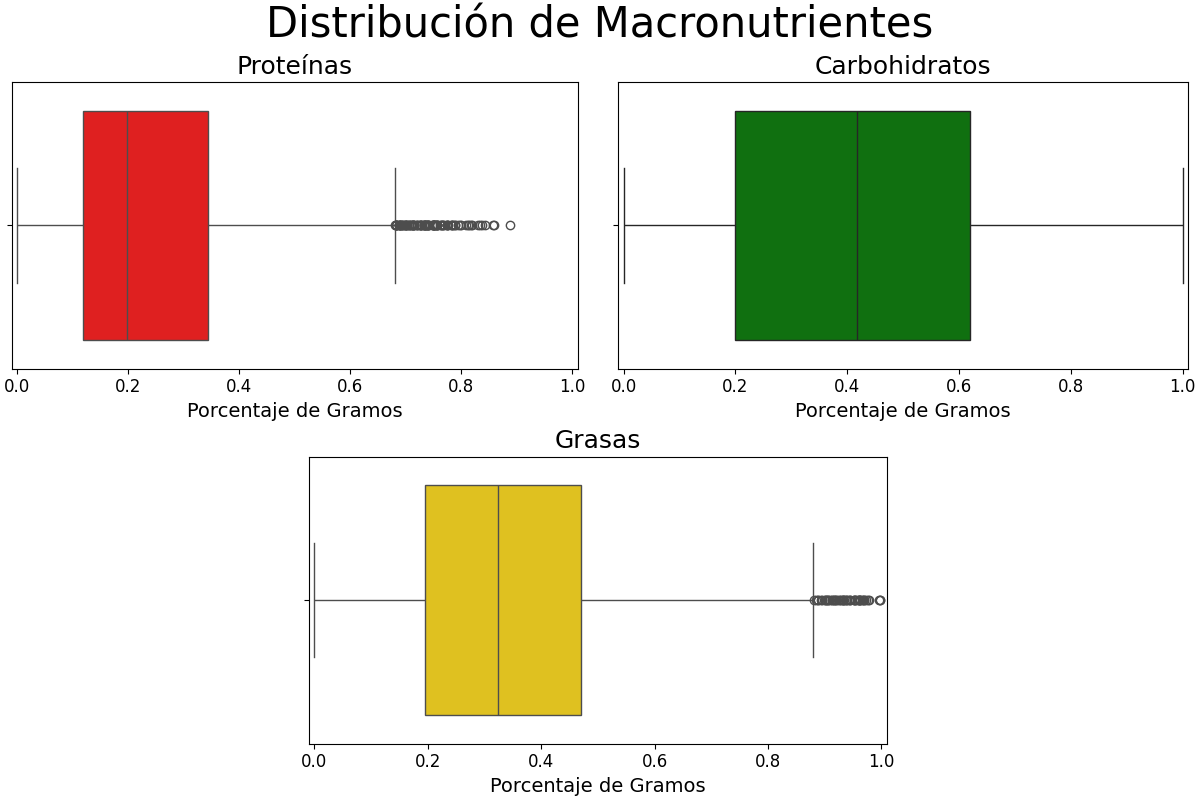
\includegraphics[width=0.9\textwidth]{Resources/EDA/VisionGeneral_1.png}
            \end{center}

            Al considerar la influencia de \emph{Cuisine\_type}, se tiene que las diferentes 
            cocinas conservan ligeros matices sobre la distribución de los macronutrientes, es 
            decir, pero por el solapamiento de las cajas y bigotes se podría esperar que no tengan 
            una diferencia significativa, indicando que las cocinas no tienen un influencia notoria 
            sobre los macronutrientes. En el tipo de cocina \emph{world} parece ser que tiene 
            un comportamiento atípico en comparación con las demás cocinas, por ello se va a 
            descartar del análisis.

            \begin{center}
                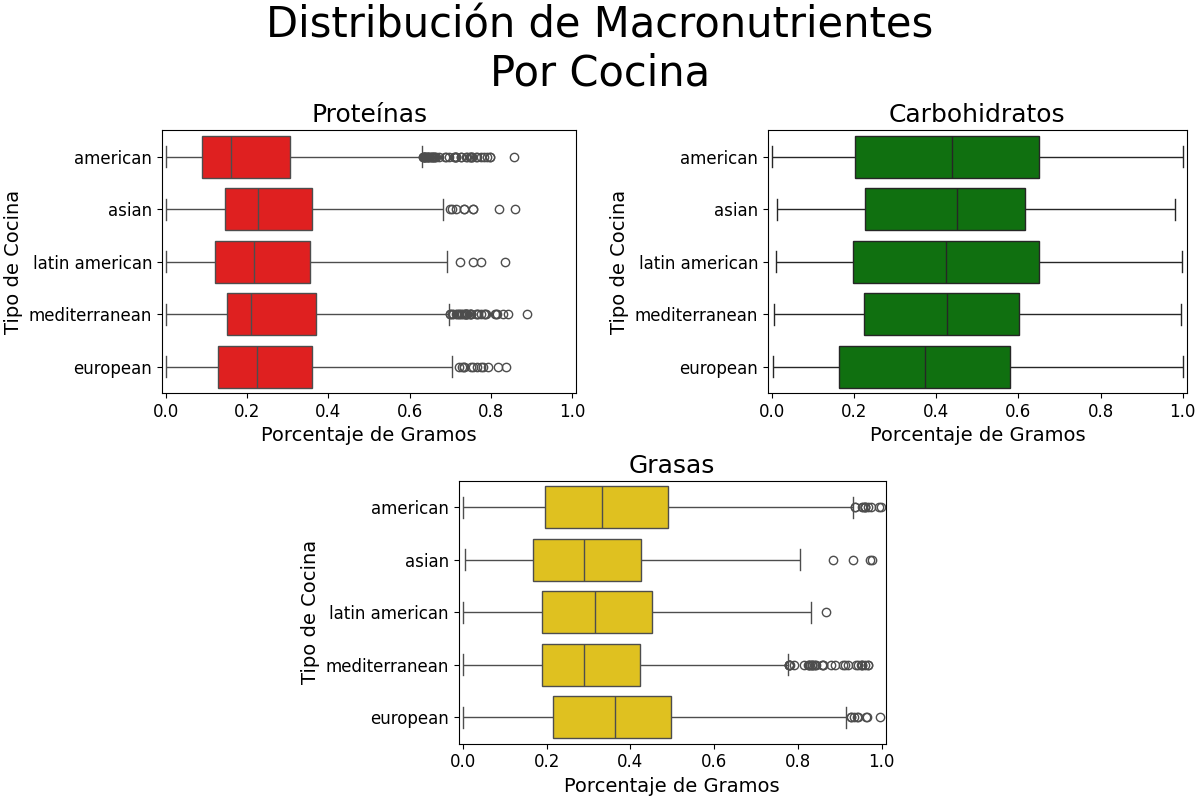
\includegraphics[width=0.9\textwidth]{Resources/EDA/VisionGeneral_2.png}
            \end{center}
        }
        
        \subsection{Dieta DASH}
        {
            Una receta de esta dieta tendrá que, en promedio, el $49\%$ de sus 
            macronutrientes son carbohidratos (provenientes de frutas, vegetales 
            y granos enteros); el $29\%$ son grasas que, por su naturaleza, son 
            saludables; y el $22\%$ son proteínas, las cuáles provienen de carnes margas.
            Aunque esta dieta se menciona ser saludable para la salud cardiovascular, 
            no implica que exista un balance o equilibrio en los macronutrientes 
            consumidos por receta. Debido a la desviación estándar y rango intercuartil de las 
            de proteínas y grasas, se tiene que estos macronutrientes se encuentran 
            concentrados en un rango más pequeño de valores en comparación con los 
            carbohidratos. De lo mencionado, podría significar que la contribución 
            de los macronutrientes no son tan variadas como lo que se esperaría 
            contradiciendo que sea una dieta saludable, notando que es una dieta 
            rica en carbohidratos. Esto no excluye que el consumir varias recetas 
            (comidas) se logré un balance.

            \begin{center}
                \begin{tabular}{l|rrr}
                \toprule
                    Medida & Carbs & Protein & Fat \\
                \midrule
                    Media               & 0.491629 & 0.220058 & 0.288313 \\
                    $Q_1$               & 0.299070 & 0.094259 & 0.159870 \\
                    $Q_2$               & 0.502760 & 0.180192 & 0.267363 \\
                    $Q_3$               & 0.683241 & 0.311076 & 0.393803 \\
                    Desviación Estándar & 0.249919 & 0.161171 & 0.182336 \\
                    Mínimo              & 0.001526 & 0.000000 & 0.000000 \\
                    Máximo              & 1.000000 & 0.833467 & 0.973404 \\
                    Asimetría de Fisher & -0.009756 & 1.029402 & 0.766955 \\
                \bottomrule
                \end{tabular}\\
                \vspace{0.5cm}
                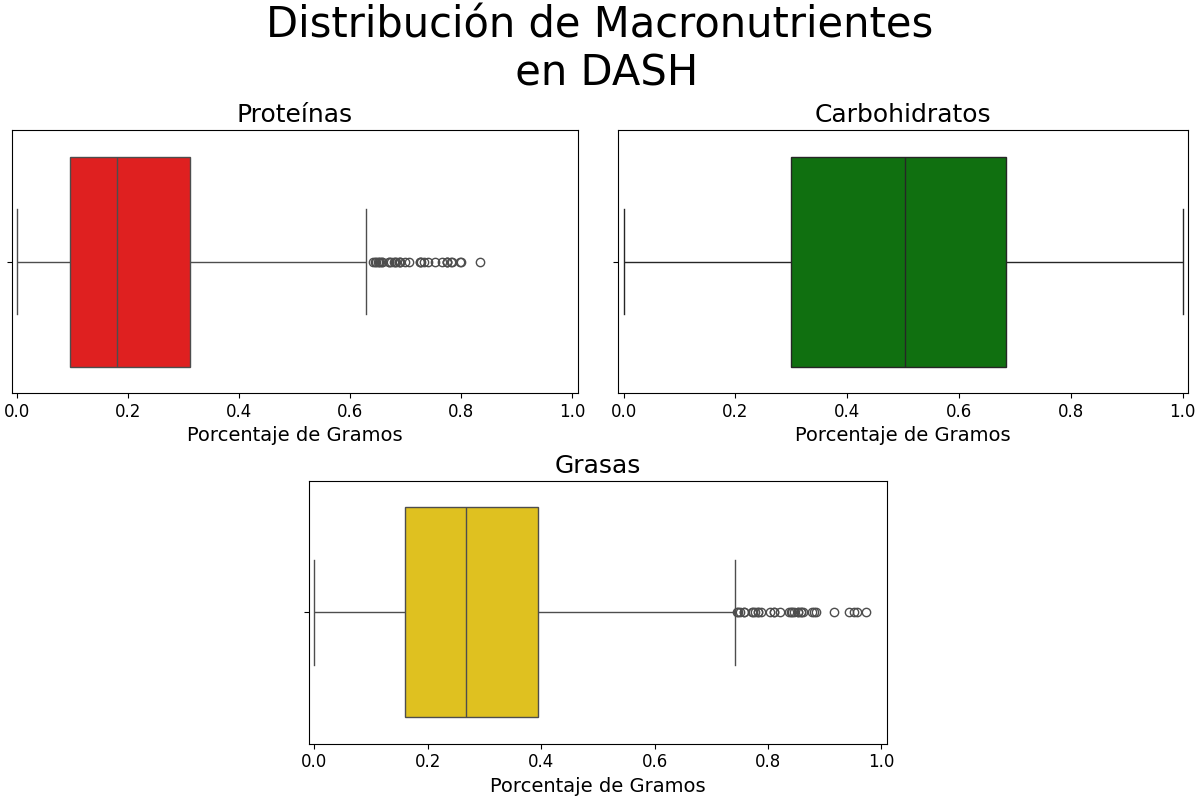
\includegraphics[width=0.9\textwidth]{Resources/EDA/Dash_1.png}
            \end{center}

            Al usar los tipos de cocina, se puede apreciar el como en cada una de 
            ellas tiene un comportamiento ligeramente diferente, es decir, al considerar 
            las cocinas en la dieta DASH se puede apreciar como los macronutrientes no 
            tienen una diferencia notoria sino que son cambios ligeros sobre su comportamiento. 
            Por ello, se puede decir que la dieta DASH es consistente sobre las cocinas y 
            que se comporta de la misma manera, aunque si se hace uso de un estadístico para 
            medir esta diferencia, tendrá un valor bajo más no será nulo.

            \begin{center}
                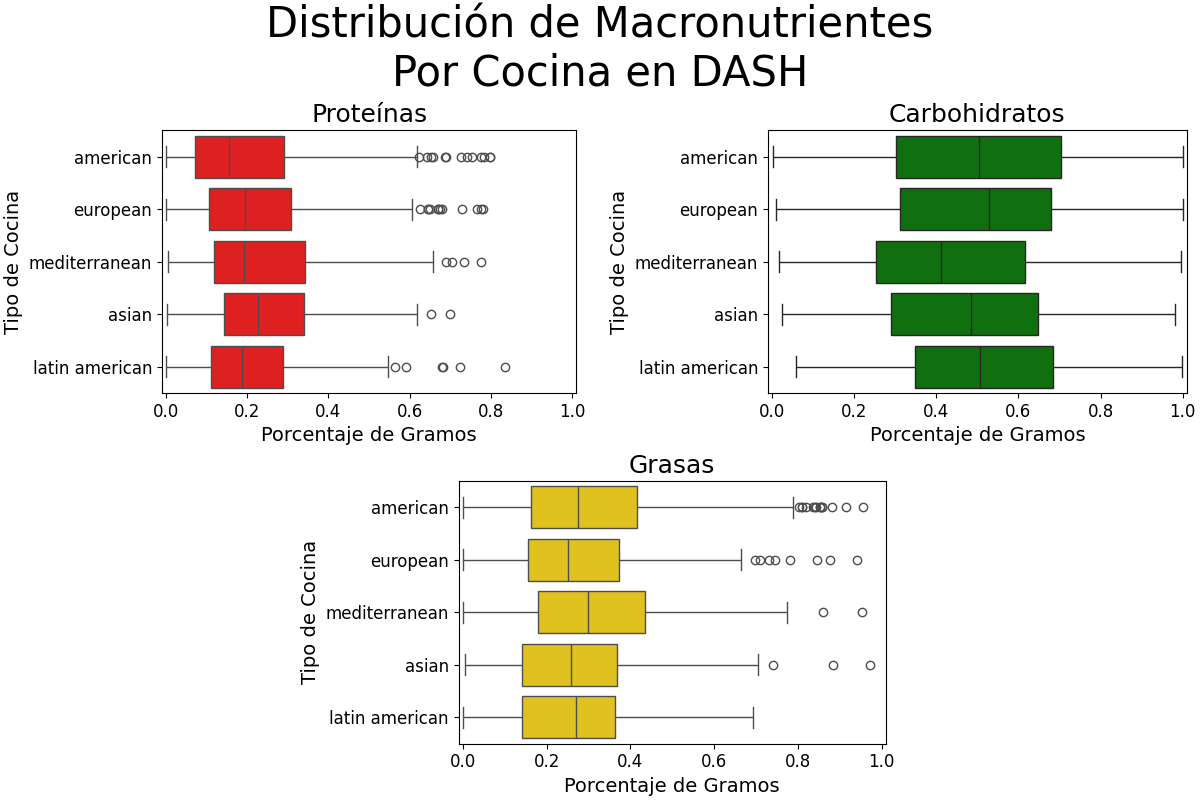
\includegraphics[width=0.9\textwidth]{Resources/EDA/Dash_2.png}
            \end{center}
        }

        \subsection{Dieta Keto}
        {
            Una receta de esta dieta tendrá que, en promedio, el $50\%$ de 
            sus macronutrientes son grasas, esto se relaciona con el hecho de 
            que se intenta inducir la ketosis (principio en que se basa esta         
            dieta); el $30\%$ son proteínas, notando que se intenta reducir 
            el consumo de carbohidratos; y el $20\%$ son carbohidratos, 
            resaltando ser una dieta baja en carbohidratos. Como la 
            proporciones de carbohidratos cuenta con un sesgo positivo, se 
            tiene que refuerza el hecho de ser una dieta baja en carbohidratos. 
            De los aportes de grasas, se observa que su sesgo es despreciable 
            implicando que existen recetas tanto con aportes altos de este 
            macronutriente (lo que se busca) mientras que hay recetas con 
            una contribución baja o nula del mismo.
        
            \begin{center}
                \begin{tabular}{l|lll}
                    \toprule
                        Medida & Carbs & Protein & Fat \\
                    \midrule
                        Media               & 0.198449 & 0.302718 & 0.498833 \\
                        $Q_1$               & 0.085336 & 0.159164 & 0.408251 \\
                        $Q_2$               & 0.156879 & 0.304214 & 0.506381 \\
                        $Q_3$               & 0.264915 & 0.410555 & 0.592312 \\
                        Desviación Estándar & 0.155979 & 0.166667 & 0.165075 \\
                        Mínimo              & 0.002060 & 0.000000 & 0.000000 \\
                        Máximo              & 1.000000 & 0.856868 & 0.997940 \\
                        Asimetría de Fisher & 1.562095 & 0.313745 & -0.120900 \\
                    \bottomrule
                \end{tabular}\\
                \vspace{0.5cm}
                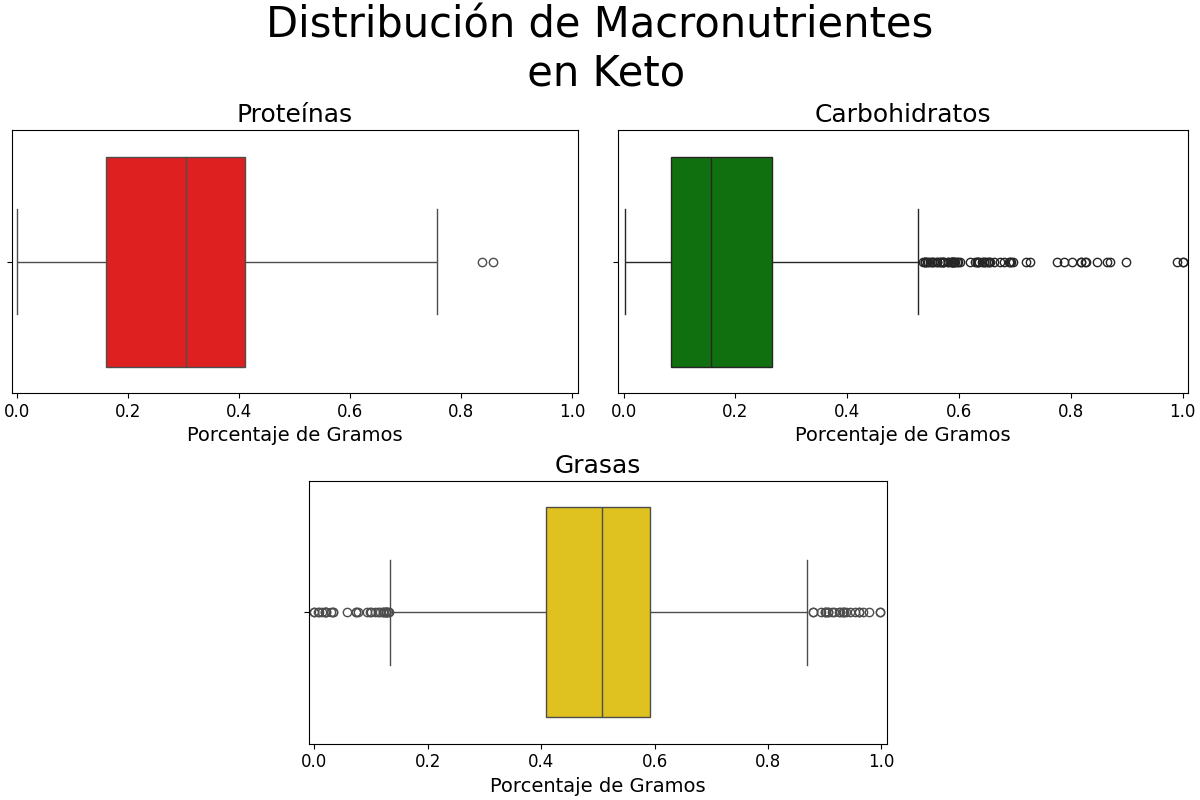
\includegraphics[width=0.9\textwidth]{Resources/EDA/Keto_1.png}
            \end{center}

            Para la dieta keto, lo más importante es mantener un consumo alto de grasas, o 
            por al menos mayor que el de carbohidratos. Por lo que al ver la distribución de 
            las grasas contra los carbohidratos en cada una de las cocinas se verifica esto, 
            per además se reportan casos, datos atípicos, donde ocurre lo contrario; omitiendo 
            esto, se puede ver como la tendencia es tener un consumo alto de grasas, aunque, por 
            ejemplo la cocina asiática, su consumo de grasas figura ser más bajo pero tienen 
            un sesgo negativo, por ello se puede determinar que sigue el principio de la dieto keto.

            \begin{center}
                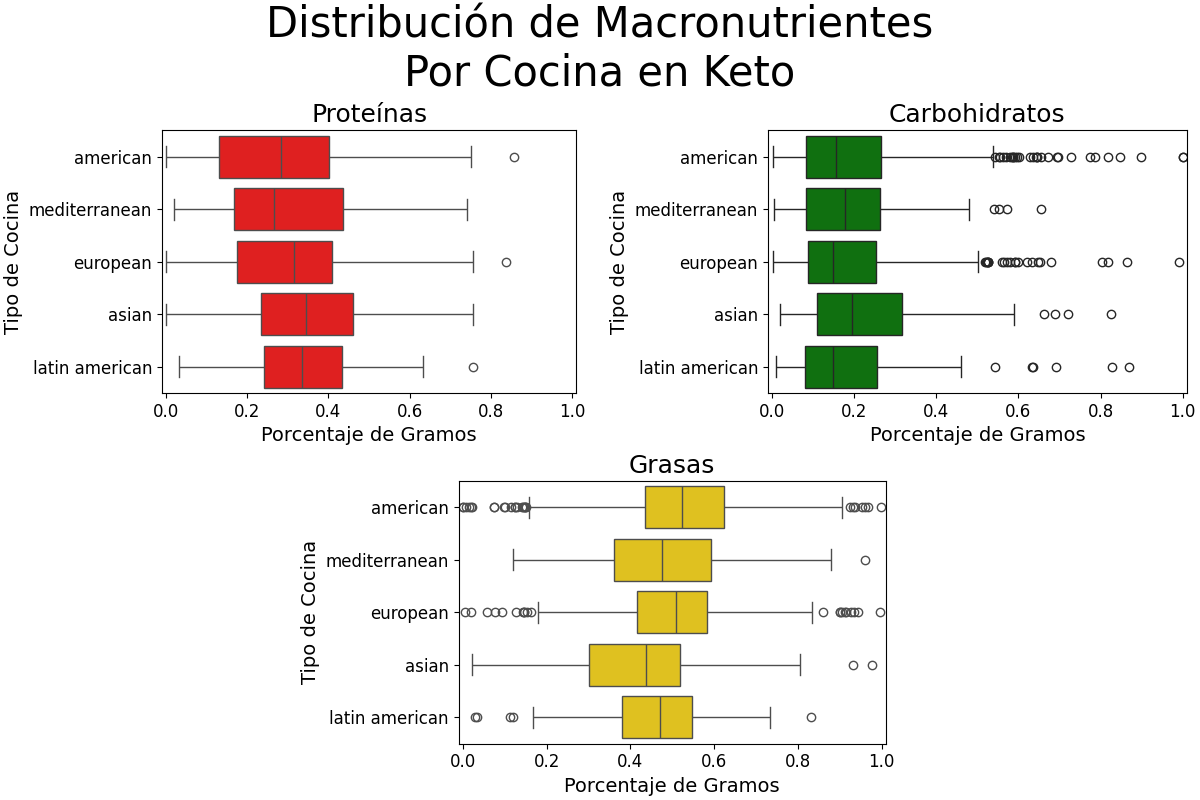
\includegraphics[width=0.9\textwidth]{Resources/EDA/Keto_2.png}
            \end{center}
        }

        \subsection{Dieta Mediterránea}
        {
            Una receta de esta dieta tendrá que, en promedio, el $42\%$ de sus 
            macronutrientes son carbohidratos, esto debido a un alto consumo de 
            productos como, frutas, vegetales y granos enteros; el $30\%$ son 
            grasas, resaltando un alto consumo de nueces y aceite de oliva, como 
            también un consumo moderado de pescado; y el $28\%$ son proteínas, 
            vinculado con un consumo moderado de pescado y aves de corral, y un 
            bajo consumo de carnes rojas. Las proteínas y grasas tienen un alto 
            sesgo positivo junto con una desviación estándar bajo, esto representa 
            que muchas de las recetas tendrán bajas proporciones de estos macronutrientes. 
            Haciendo que se comporte de forma análoga que la dieta DASH pero incluso 
            hasta más balanceada.\\

            \begin{center}
                \begin{tabular}{l|lll}
                    \toprule
                        Medida & Carbs & Protein & Fat \\
                    \midrule
                        Media               & 0.422803 & 0.280190 & 0.297007 \\
                        $Q_1$               & 0.249507 & 0.159930 & 0.180738 \\
                        $Q_2$               & 0.438382 & 0.229058 & 0.268950 \\
                        $Q_3$               & 0.605733 & 0.377918 & 0.390790 \\
                        Desviación Estándar & 0.212640 & 0.162485 & 0.160349 \\
                        Mínimo              & 0.006733 & 0.005036 & 0.001731 \\
                        Máximo              & 0.992746 & 0.887557 & 0.968722 \\
                        Asimetría de Fisher & -0.123218 & 0.962969 & 0.878710 \\
                    \bottomrule
                \end{tabular}\\
                \vspace{0.5cm}
                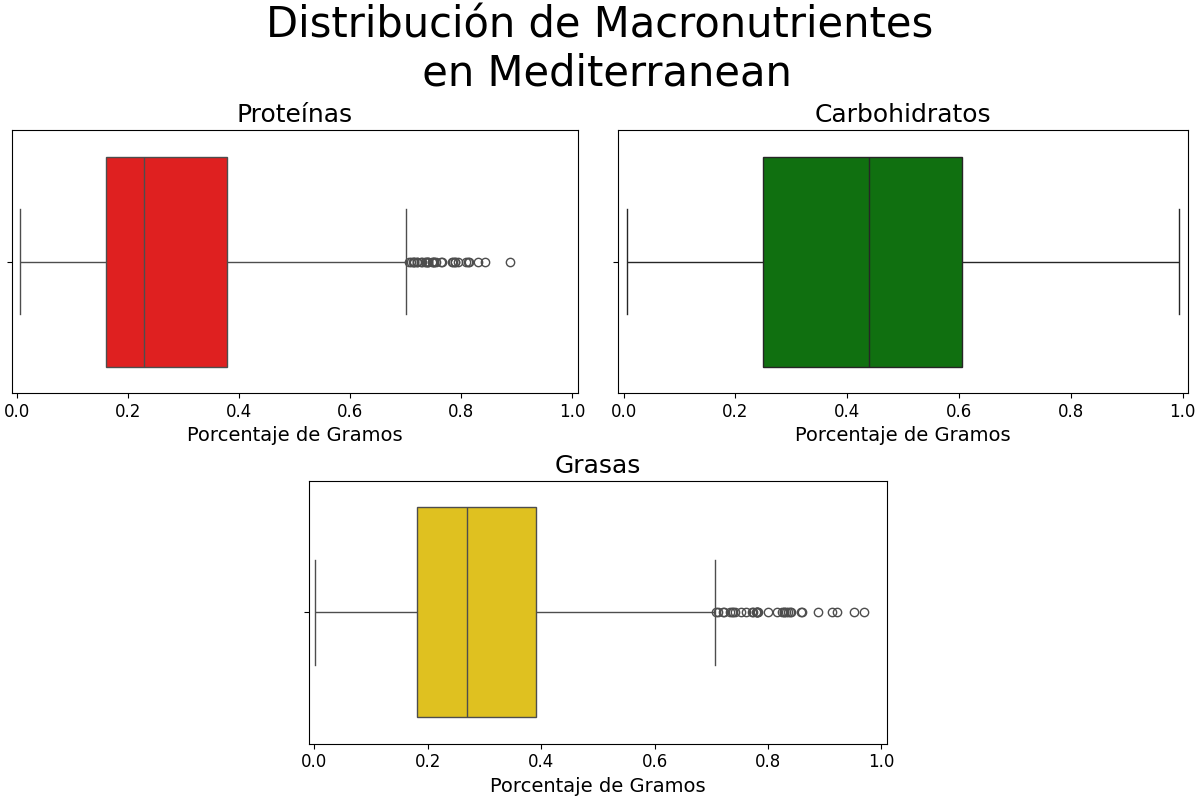
\includegraphics[width=0.9\textwidth]{Resources/EDA/Mediterranean_1.png}
            \end{center}       

            Debido que para esta receta se cuenta con la región de dónde proviene, la 
            comparativa se vuelve respecto a la distribución de los macronutrientes en 
            la cocina del mediterráneo. Se tiene que las grasas se encuentran más variadas, 
            es decir, en las cocinas diferentes a la mediterránea se puede ver que en 
            algunas cocinas toman valores más altos o más bajos en las grasas. Al considerar 
            las proteínas se puede apreciar este mismo fenómeno pero en menor medida, debido 
            a que puede existir una diversificación de la dieta para adecuarse a los 
            productos y alimentos propios de una cierta región.

            \begin{center}
                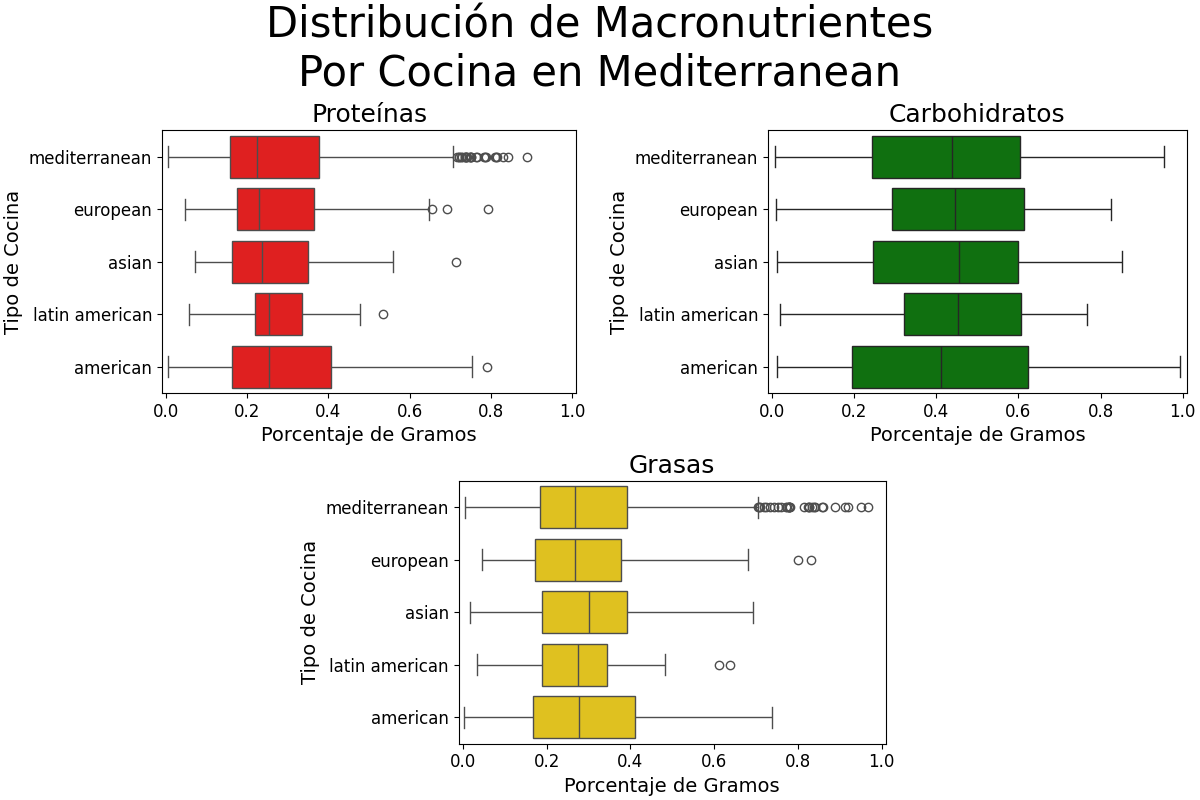
\includegraphics[width=0.9\textwidth]{Resources/EDA/Mediterranean_2.png}
            \end{center}
        }

        \subsection{Dieta Paleo}
        {
            Una receta de esta dieta tendrá que, en promedio, el $38\%$ de sus 
            macronutrientes son grasas y el $37\%$ son carbohidratos, esto se 
            relaciona con el consumo de productos como frutas, vegetales, nueces 
            y semillas; y el $25\%$ son proteínas cuyas principales fuentes son 
            carnes margas y pescado. La posible limitante de alimentos asociados 
            a proteínas	y grasas podría impactar en que las recetas estén hechas 
            con los mismos productos dentro de la misma región geográfica. Estos 
            se relacionaría con una baja variedad en la presencia de estos 
            macronutrientes, esto podría incluso explicar que las desviaciones 
            estándar se parezcan entre sí.\\

            \begin{center}
                \begin{tabular}{l|lll}
                    \toprule
                        Medida & Carbs & Protein & Fat \\
                    \midrule
                        Media               & 0.369912 & 0.250207 & 0.379881 \\
                        $Q_1$               & 0.191815 & 0.103933 & 0.257510 \\
                        $Q_2$               & 0.350726 & 0.207286 & 0.382872 \\
                        $Q_3$               & 0.512822 & 0.375863 & 0.488153 \\
                        Desviación Estándar & 0.219894 & 0.174915 & 0.174737 \\
                        Mínimo              & 0.003612 & 0.000000 & 0.006210 \\
                        Máximo              & 0.976322 & 0.858503 & 0.968835 \\
                        Asimetría de Fisher & 0.473617 & 0.710366 & 0.325286 \\
                    \bottomrule
                \end{tabular}\\
                \vspace{0.5cm}
                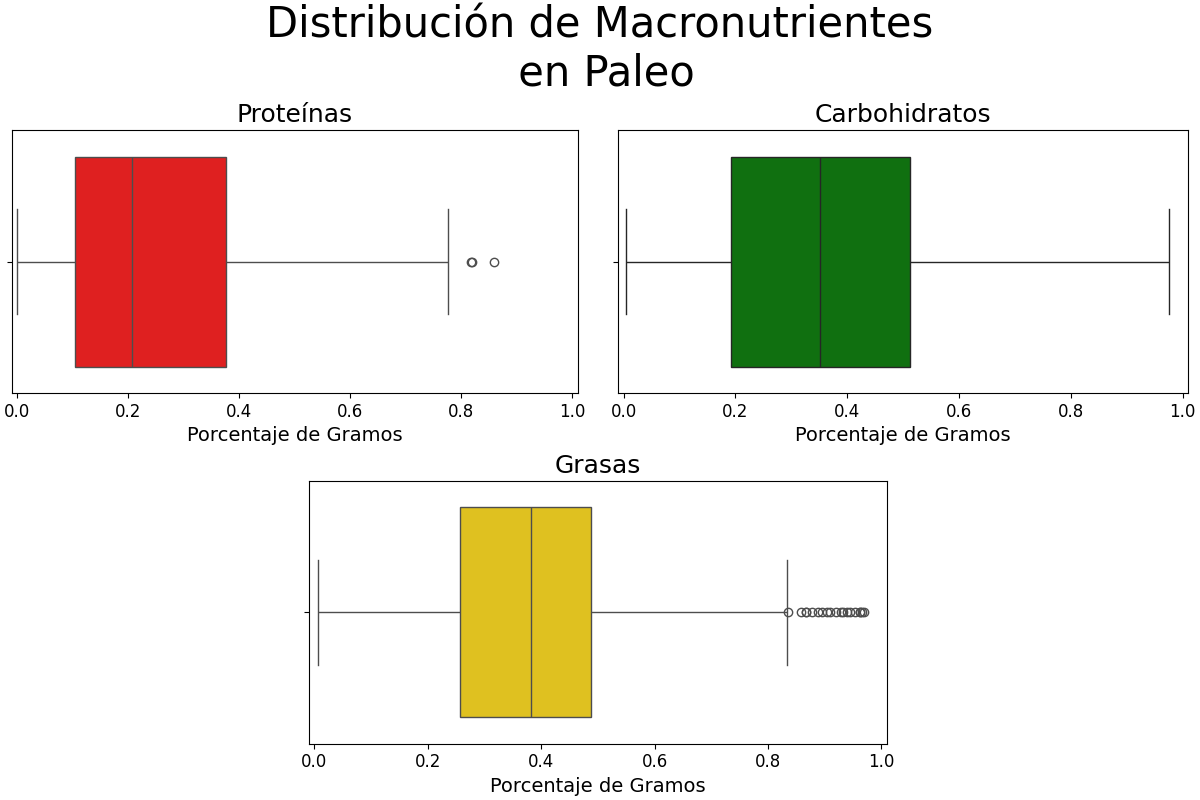
\includegraphics[width=0.9\textwidth]{Resources/EDA/Paleo_1.png}
            \end{center}       

            Que las proteínas y grasas tengan distribuciones diferentes entre 
            las cocinas se relaciona con el hecho de que cada región geográfica 
            tiene diferentes disponibilidad de recursos alimentarios, haciendo que 
            este fenómeno impacte en las recetas que se pueden hacer con lo que 
            esté disponible.

            \begin{center}
                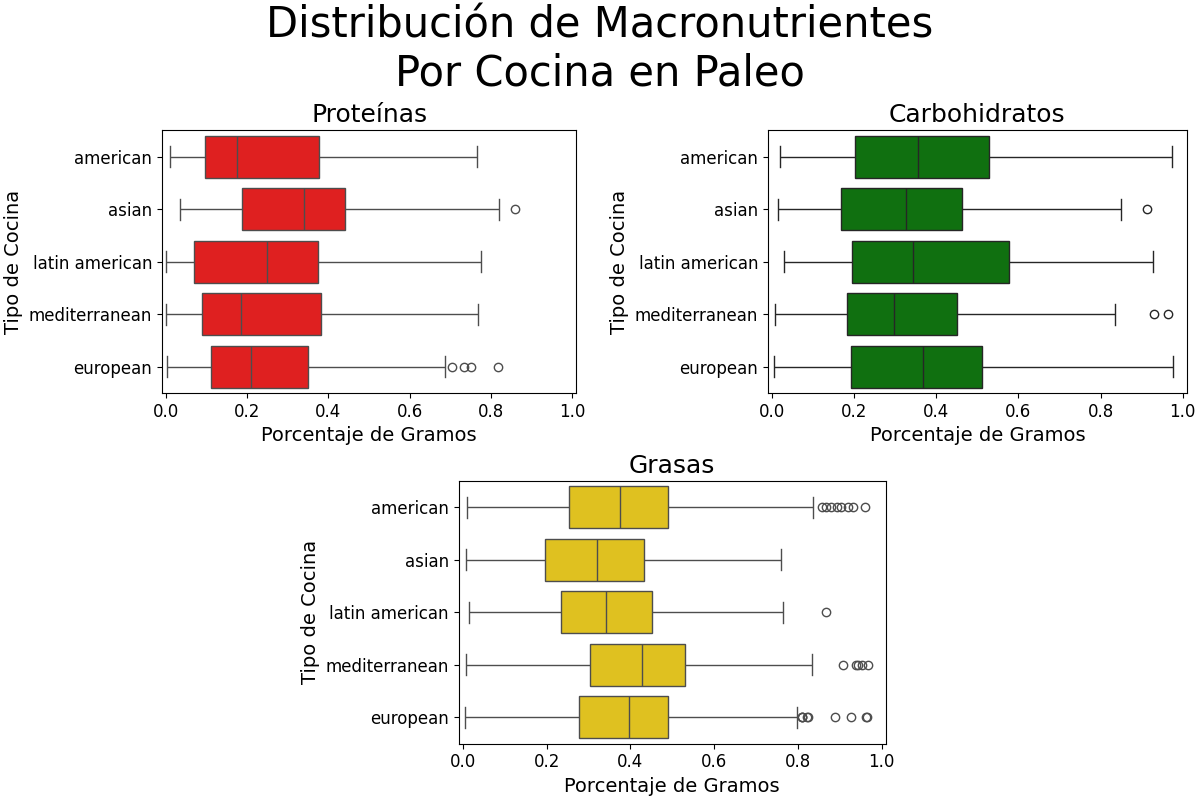
\includegraphics[width=0.9\textwidth]{Resources/EDA/Paleo_2.png}
            \end{center}
        }

        \subsection{Dieta Vegana}
        {
            Una receta de esta dieta tendrá que, en promedio, el $60\%$ de 
            sus macronutrientes son carbohidratos, que provienen de fuentes 
            como vegetales, frutas, cereales y legumbres; el $25\%$ son grasas, 
            relacionadas con el consumo de nueces y semillas; y el $15\%$ son 
            proteínas, esto debido a un nulo consumo de alimentos de origen 
            animal y que estas fuentes son reemplazadas por fuentes vegetales. 
            En las proteínas, se puede observar un rango intercuartil reducido y una 
            desviación estándar reducida, esto evoca a que las recetas tengan bajos 
            aportes de proteínas así como también los valores de aportes se concentren 
            en un rango reducido.\\

            \begin{center}
                \begin{tabular}{l|lll}
                    \toprule
                        Medida & Carbs & Protein & Fat \\
                    \midrule
                        Media               & 0.593169 & 0.148801 & 0.258029 \\
                        $Q_1$               & 0.502866 & 0.085853 & 0.143034 \\
                        $Q_2$               & 0.625406 & 0.139807 & 0.231985 \\
                        $Q_3$               & 0.713660 & 0.190724 & 0.344991 \\
                        Desviación Estándar & 0.171149 & 0.086151 & 0.160262 \\
                        Mínimo              & 0.000330 & 0.001921 & 0.000112 \\
                        Máximo              & 0.986872 & 0.647416 & 0.994887 \\
                        Asimetría de Fisher & -0.735666 & 1.439623 & 1.092007 \\
                    \bottomrule
                \end{tabular}\\
                \vspace{0.5cm}
                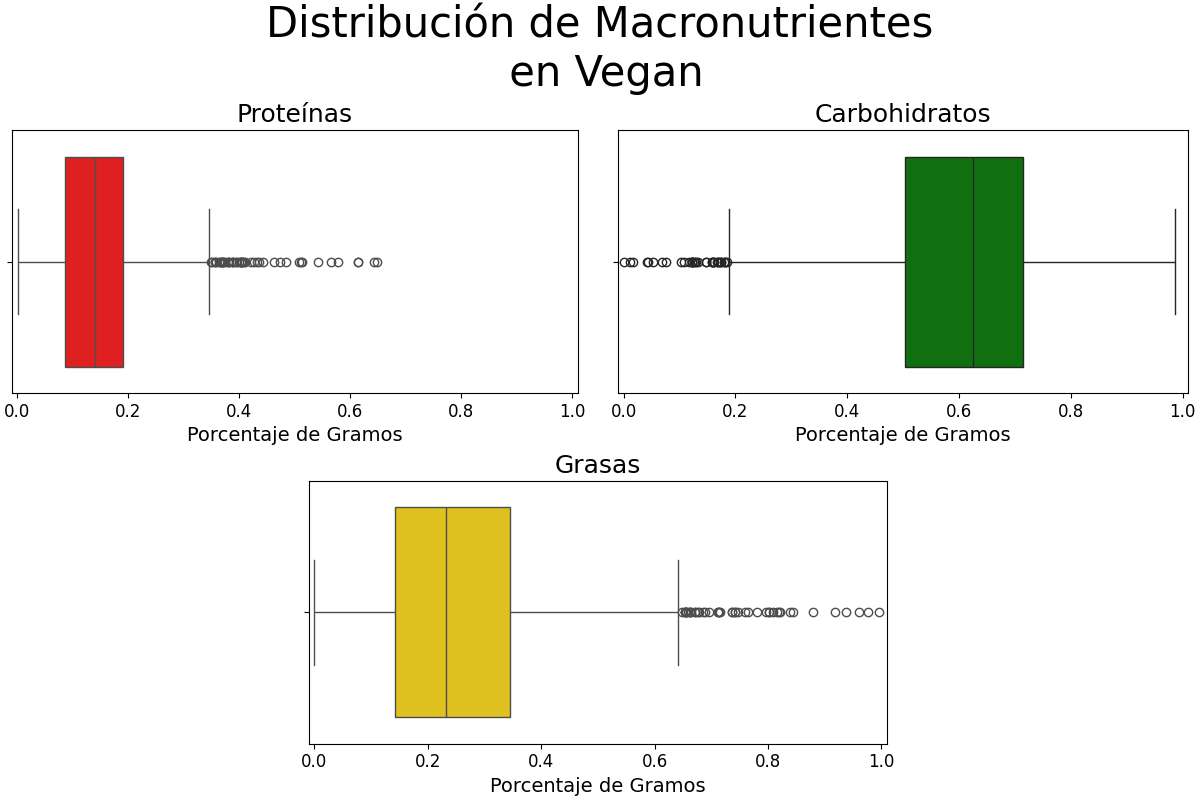
\includegraphics[width=0.9\textwidth]{Resources/EDA/Vegan_1.png}
            \end{center}       

            Se tiene que entre las cocinas se encuentran diferencias en las 
            proteínas y carbohidratos, representando que las distinciones sobre 
            las dietas se haya que tan favorecidas son las proteínas, es decir, 
            en qué cocinas se pueden encontrar alimentos con altos aportes de proteínas, 
            como lo sería la asiática que también es la que sus aportes de carbohidratos 
            tienden a ser bajos. 

            \begin{center}
                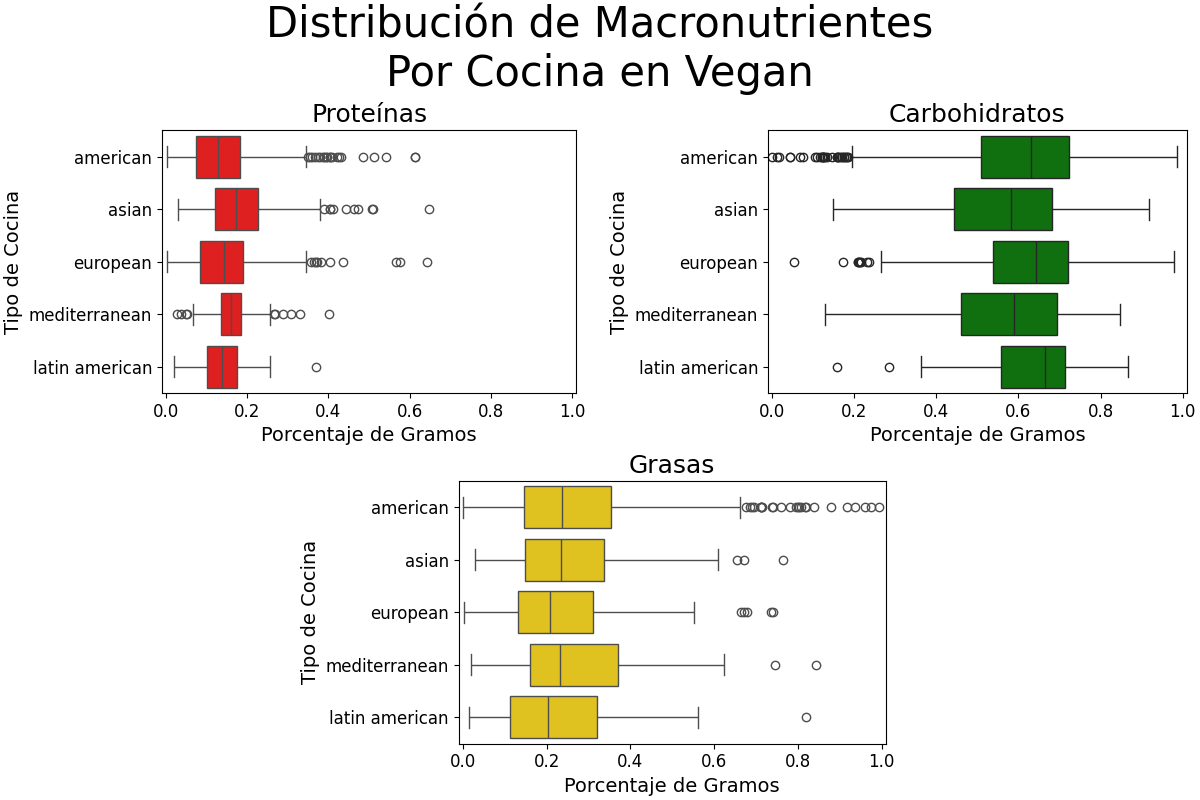
\includegraphics[width=0.9\textwidth]{Resources/EDA/Vegan_2.png}
            \end{center}   
        }
    }

    \newpage

    \section{Análisis Bivariado}\label{sec:biva}
    {
        El realizar un análisis bivariado usando todas las dietas va a 
        provocar una desvanecimiento de la información debido a que las dietas 
        tienen comportamientos heterogéneas; 
        donde de nuevo se muestra que cada dieta sigue ciertos patrones 
        y tendencias en sus macronutrientes. Debido a que los valores 
        de los macronutrientes suman $1$ se tiene que el incrementar 
        un macronutriente hace que los otros decrezcan, por lo que el 
        valor de la correlación refleja esta fuerza en que decrece o, 
        en ciertos casos, crece. En la mayoría de los casos se tienen 
        correlaciones mayores a $0.5$ en valor absoluto, esto representa 
        que son tendencias fuertes que tienen las diferentes dietas sobre 
        la composiciones de sus macronutrientes. Se tiene que la relación 
        entre carbohidratos contra proteínas y grasas permite describir de 
        otra manera cada dieta. \anexoref{anexo:B.1}

        \begin{center}
            \begin{tabular}{lllrr}
            \toprule
                Dieta & Macronutrientes & Centroide & Covarianza & \makecell{Coeficiente\\Correlación} \\
            \midrule
                dash          & (Carbs,Protein) & [0.4916 0.2200] & -0.0275 & -0.6850 \\
                dash          & (Carbs,Fat)     & [0.4916 0.2883] & -0.0348 & -0.7650 \\
                dash          & (Protein,Fat)   & [0.2200 0.2883] &  0.0016 &  0.0550 \\
                keto          & (Carbs,Protein) & [0.1984 0.3027] & -0.0124 & -0.4780 \\
                keto          & (Carbs,Fat)     & [0.1984 0.4988] & -0.0119 & -0.4621 \\
                keto          & (Protein,Fat)   & [0.3027 0.4988] & -0.0153 & -0.5578 \\
                mediterranean & (Carbs,Protein) & [0.4228 0.2801] & -0.0229 & -0.6643 \\
                mediterranean & (Carbs,Fat)     & [0.4228 0.2970] & -0.0222 & -0.6529 \\
                mediterranean & (Protein,Fat)   & [0.2801 0.2970] & -0.0034 & -0.1323 \\
                paleo         & (Carbs,Protein) & [0.3699 0.2502] & -0.0242 & -0.6293 \\
                paleo         & (Carbs,Fat)     & [0.3699 0.3798] & -0.0241 & -0.6284 \\
                paleo         & (Protein,Fat)   & [0.2502 0.3798] & -0.0063 & -0.2089 \\
                vegan         & (Carbs,Protein) & [0.5931 0.1488] & -0.0055 & -0.3740 \\
                vegan         & (Carbs,Fat)     & [0.5931 0.2580] & -0.0237 & -0.8668 \\
                vegan         & (Protein,Fat)   & [0.1488 0.2580] & -0.0019 & -0.1381 \\
            \bottomrule
            \end{tabular}
        \end{center}
        
        El tabular el coeficiente de correlación para cada par de macronutrientes y dieta, 
        se permite observar con mayor detenimiento que todos los valores son diferentes y,  
        por la cantidad de instancias por dieta, es significativo. Con ello, se tiene que 
        los macronutrientes tendrán diferentes comportamientos según la dieta a la que 
        pertenezcan. Esto implica que las dietas van a favorecer más a ciertas combinaciones 
        entre macronutrientes, y esto se relaciona con los alimentos y productos que son 
        consumidos dentro de cada dieta, así como también las cantidades; con ello, se 
        muestra que se puede determinar cuál es la dieta que favorece un cierto macronutriente 
        más que las otras.
    }

    \newpage

    \section{Muestreo e Intervalos de Confianza}
    {
        Como las tres variables cuantitativas tienen el mismo nivel 
        de relevancia, se opta por usar los \emph{Carbs} como atributo 
        para el Muestreo. Y para ambos muestreos se realizan de 
        tamaño $50$ y, usando la Regla de Sturges, se emplean 7 clases 
        o bins para la tabla de frecuencias.

        \subsection{Muestreo Simple Aleatorio}\label{subsec:sample_rand}
        {
            Al considerar los estadísticos muestrales se puede 
            apreciar que difieren en todos las medidas, por lo que este muestreo 
            no es representativo del conjunto de datos, es decir, siguen diferentes 
            distribuciones principalmente al usar la media y los cuartiles. Por lo 
            tanto, o se puede cambiar de estrategia o usar una tamaño de muestreo 
            más grande.

            \begin{center}
                \begin{tabular}{ccccc}
                        \multicolumn{5}{c}{Resultados del Muestreo} \\ 
                    \midrule
                        0.780289 &   0.15143502 & 0.13749852 &  0.60841622 & 0.69139498 \\ 
                        0.04172702 & 0.44570519 & 0.74317898 & 0.53322363 & 0.23569666\\
                        0.20240863 & 0.55306465 & 0.98825124 &  0.62201877 & 0.08367046 \\ 
                        0.7226847 & 0.53068409 & 0.10743335 & 0.06312504 & 0.75586 \\
                        0.69076424 & 0.18063042 & 0.14876349 &  0.76112551 & 0.61451786 \\ 
                        0.81901361 & 0.61532896 & 0.22294326 & 0.58007183 & 0.66899583\\
                        0.69092336 & 0.13819862 & 0.08259526 &  0.37709587 & 0.17925896 \\ 
                        0.48040837 & 0.98382353 & 0.49527076 & 0.1451375 &  0.19026882\\
                        0.63525297 & 0.44261674 & 0.22074399 &  0.41293142 & 0.60653006 \\ 
                        0.55742063 & 0.42509449 & 0.19835071 & 0.45468297 & 0.3959553\\
                \end{tabular}
            \end{center}

            \begin{center}
                \begin{tabular}{lrrrr}
                \toprule
                    \makecell{Marca de\\Clase} & \makecell{Frecuencia\\Abosluta} & \makecell{Frecuencias\\Relativa} & \makecell{Frecuencia\\Acumuladas} & z-score \\
                \midrule
                    0.109336 & 10 & 0.20 & 0.20 & -1.308939 \\
                    0.244554 & 8  & 0.16 & 0.36 & -0.786707 \\
                    0.379771 & 6  & 0.12 & 0.48 & -0.264474 \\
                    0.514989 & 8  & 0.16 & 0.64 &  0.257759 \\
                    0.650207 & 10 & 0.20 & 0.84 &  0.779991 \\
                    0.785425 & 6  & 0.12 & 0.96 &  1.302224 \\
                    0.920642 & 2  & 0.04 & 1.00 &  1.824456 \\
                \bottomrule
                \end{tabular}
            \end{center}

            \begin{minipage}{0.35\textwidth}
                \centering
                \begin{tabular}{l|r}
                \toprule
                    Medida Muestral & Carbs \\
                \midrule
                    Media               & 0.448250 \\
                    $Q_1$               & 0.192289 \\
                    $Q_2$               & 0.467546 \\
                    $Q_3$               & 0.631944 \\
                    Desviación Estándar & 0.258922 \\
                    Mínimo              & 0.041727 \\
                    Máximo              & 0.988251 \\
                    Asimetría de Fisher & 0.088215 \\
                \bottomrule
                \end{tabular}
            \end{minipage}%
            \begin{minipage}{0.65\textwidth}
                \centering
                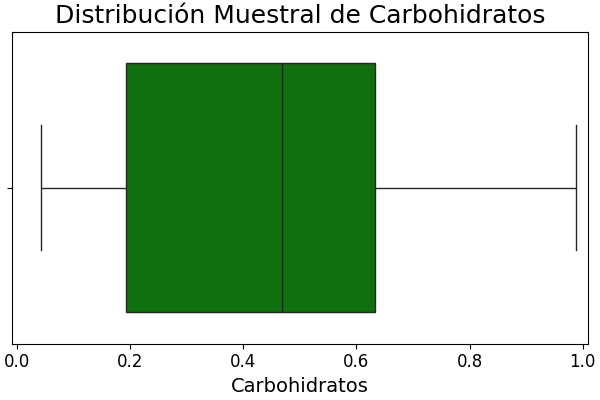
\includegraphics[width=0.9\textwidth]{Resources/Sampling/Random.png}
            \end{minipage}
        }

        \subsection{Muestreo Aleatorio Estratificado}
        {
            Al igual que en \fullref{subsec:sample_rand}, se tiene que en el muestreo 
            estratificado no es representativo del conjunto de datos, esto se deriva 
            del hecho de que las medidas muestrales difieren notoriamente de las poblacionales 
            y además de seguir una distribución diferente. Con ello, se tiene que la solución 
            para obtener un muestreo representativo se vuelve justamente incrementar 
            el tamaño de la muestra.

            \begin{center}
                \begin{tabular}{ccccc}
                        \multicolumn{5}{c}{Resultados del Muestreo} \\ 
                    \midrule
                        0.98825124 & 0.44840909 & 0.89960239 & 0.83874942 & 0.365615   \\
                        0.49887176 & 0.58630187 & 0.3157274  & 0.5842796  & 0.57451464 \\
                        0.08873597 & 0.68983711 & 0.16884721 & 0.15916624 & 0.09565607 \\
                        0.52595787 & 0.07693278 & 0.27939369 & 0.12009859 & 0.22105597 \\
                        0.45648684 & 0.56049479 & 0.57414311 & 0.28213503 & 0.61598047 \\
                        0.56339749 & 0.52937621 & 0.5663925  & 0.65277566 & 0.2666113  \\
                        0.13609793 & 0.41432132 & 0.13118082 & 0.07637211 & 0.17604633 \\
                        0.77068989 & 0.52892388 & 0.39944097 & 0.13687658 & 0.00708689 \\
                        0.6840657  & 0.32537609 & 0.3360161  & 0.50114789 & 0.89117851 \\
                        0.65409493 & 0.30271941 & 0.80744214 & 0.60015393 & 0.65224341 \\
                \end{tabular}
            \end{center}

            \begin{center}
                \begin{tabular}{lrrrr}
                \toprule
                    \makecell{Marca de\\Clase} & \makecell{Frecuencia\\Abosluta} & \makecell{Frecuencias\\Relativa} & \makecell{Frecuencia\\Acumuladas} & z-score \\
                \midrule
                    0.077170 &  9 & 0.18 & 0.18 & -1.457119 \\
                    0.217336 &  7 & 0.14 & 0.32 & -0.898073 \\
                    0.357503 &  7 & 0.14 & 0.46 & -0.339028 \\
                    0.497669 & 10 & 0.20 & 0.66 & 0.220017 \\
                    0.637835 & 11 & 0.22 & 0.88 & 0.779062 \\
                    0.778002 &  3 & 0.06 & 0.94 & 1.338107 \\
                    0.918168 &  3 & 0.06 & 1.00 & 1.897152 \\
                \bottomrule
                \end{tabular}
            \end{center}

            \begin{minipage}{0.35\textwidth}
                \centering
                \begin{tabular}{l|r}
                \toprule
                    Medida Muestral & Carbs \\
                \midrule
                    Media               & 0.442505 \\
                    $Q_1$               & 0.232445 \\
                    $Q_2$               & 0.477679 \\
                    $Q_3$               & 0.596691 \\
                    Desviación Estándar & 0.250725 \\
                    Mínimo              & 0.007087 \\
                    Máximo              & 0.988251 \\
                    Asimetría de Fisher & 0.129906 \\
                \bottomrule
                \end{tabular}
            \end{minipage}%
            \begin{minipage}{0.65\textwidth}
                \centering
                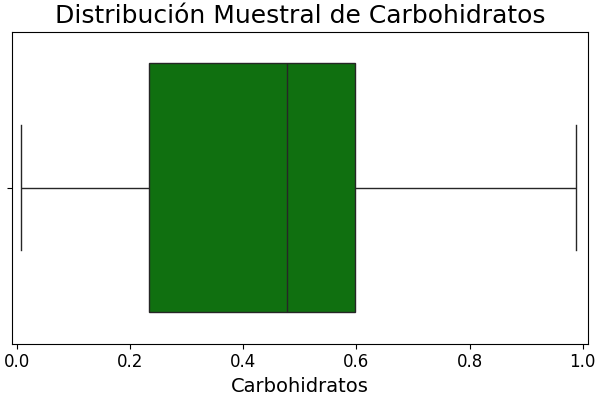
\includegraphics[width=0.9\textwidth]{Resources/Sampling/Stratified.png}
            \end{minipage}
        }
    
        \subsection{Intervalos de Confianza}
        {
            En cada muestreo, se determina los intervalos 
            con los niveles de confianza del $85\%$, $95\%$ y $99\%$, 
            y en cada intervalo se determinó si la media poblacional de 
            los carbohidratos pertenece al intervalo construido. De los 
            intervalos de confianza construidos, se tiene que en todos
            pertenece la media poblacional.\\

            \begin{minipage}{0.5\textwidth}
                \centering
                \begin{tabular}{r|rr}
                    \multicolumn{3}{c}{Muestreo Simple Aleatorio} \\
                \midrule
                    \makecell{Nivel de\\Confianza} & \makecell{Límite\\Inferior} & \makecell{Límite\\Superior} \\
                \midrule
                    $85\%$ & 0.395538 & 0.500961 \\
                    $95\%$ & 0.376481 & 0.520018 \\
                    $99\%$ & 0.353930 & 0.542569 \\
                \bottomrule
                \end{tabular}
            \end{minipage}% 
            \begin{minipage}{0.5\textwidth}
                \centering
                \begin{tabular}{r|rr}
                    \multicolumn{3}{c}{Muestreo Aleatorio Estratificado} \\
                \midrule
                    \makecell{Nivel de\\Confianza} & \makecell{Límite\\Inferior} & \makecell{Límite\\Superior} \\
                \midrule
                    $85\%$ & 0.391463 & 0.493548 \\
                    $95\%$ & 0.373009 & 0.512001 \\
                    $99\%$ & 0.351172 & 0.533839 \\
                \bottomrule
                \end{tabular}
            \end{minipage}
        }
    }

    \newpage

    \section{Pruebas de Hipótesis}
    {

    }

    \addcontentsline{toc}{section}{Anexos}
    \appendix
    {
        \section{Marco Teórico}\label{anexo:A}
        {
        La dieta es uno de los principales factores de riesgo de las enfermedades 
        crónicas, y las enfermedades sensibles a la dieta contribuyen en gran medida 
        a los costes sanitarios mundiales. Se han propuesto literalmente miles de 
        \emph{dietas}, que pueden describirse en términos generales como basadas en 
        creencias, en alimentos específicos o en nutrientes; centradas en la 
        pérdida de peso o en el aumento de peso (muscular); dietas de desintoxicación 
        (detox) y dietas diseñadas por razones médicas específicas.\cite{marvastipopular} \\
        
        Las \emph{dietas de moda} son dietas populares durante un tiempo sin basarse 
        necesariamente en una recomendación dietética estándar. A menudo promueven 
        una pérdida de peso irracionalmente rápida o afirmaciones de salud sin 
        sentido, y se anuncian como dietas que requieren poco esfuerzo por parte de 
        quien las sigue. La promesa de ganancias fáciles, combinada con la presión 
        social para lograr un determinado tipo de cuerpo, puede dejar al público 
        susceptible a afirmaciones infundadas o exageradas.\cite{marvastipopular} \\
        
        Las dietas estudiadas desde una perspectiva estadística en el presente 
        trabajo, son englobadas en las \emph{dietas de moda}, que a veces son referidas 
        como \emph{dietas sin evidencia científica}. Siendo  la dieta DASH la única 
        que cuenta con algún tipo de fundamento.
        
        \subsection{DASH (Dietary Approaches to Stop Hypertension)}
        {
            \cite{marvastipopular} La dieta DASH (Enfoques Dietéticos para Detener la 
            Hipertensión) es un patrón dietético diseñado específicamente para ayudar 
            a reducir la presión arterial y promover la salud general del corazón. Hace 
            hincapié en el consumo de una variedad de alimentos ricos en nutrientes, 
            como frutas, verduras, cereales integrales, proteínas magras y productos 
            lácteos bajos en grasa, y en la limitación de la ingesta de sodio, grasas 
            saturadas y azúcares añadidos. 
        }
            
        \subsection{Dieta Keto}
        {
            \cite{marvastipopular} Una dieta baja en hidratos de carbono (baja en 
            carbohidratos) es un patrón alimentario que restringe la ingesta de 
            carbohidratos, sustituyéndolos normalmente por mayores cantidades de 
            proteínas y grasas. La dieta cetogénica es una forma de dieta baja en 
            carbohidratos con un alto contenido en grasas en relación con la ingesta 
            de proteínas y carbohidratos.\\
            
            El objetivo de la dieta cetogénica es inducir la cetosis, un estado 
            metabólico que se produce cuando el cuerpo quema grasa para obtener 
            energía en lugar de glucosa, lo que induce la pérdida de peso.
        }
                
        \subsection{Dieta Mediterránea}
        {
            \cite{marvastipopular} La dieta mediterránea es un patrón alimentario 
            inspirado en los hábitos alimenticios tradicionales de los países 
            situados a orillas del mar Mediterráneo. Se caracteriza por un alto consumo 
            de frutas, verduras, cereales integrales, legumbres, frutos secos y 
            aceite de oliva; un consumo moderado de pescado y aves; y un bajo 
            consumo de carnes rojas, alimentos procesados y dulces.
        }
                    
        \subsection{Dieta Paleo (Paleolítica)}
        {
            \cite{marvastipopular} La dieta paleo, también conocida como dieta 
            paleolítica o dieta del hombre de las cavernas, es un enfoque 
            dietético que pretende imitar los hábitos alimentarios de nuestros 
            antiguos antepasados del Paleolítico. \\
            
            Hace hincapié en el consumo de alimentos integrales y no procesados 
            que habrían estado al alcance de los primeros humanos, como carnes magras, 
            pescado, frutas, verduras, frutos secos y semillas, y excluye los cereales, 
            las legumbres, los productos lácteos, los alimentos procesados y los 
            azúcares añadidos.
        }
        
        \subsection{Dieta Vegana}
        {
            \cite{marvastipopular} La dieta vegana es un patrón dietético basado en 
            plantas que excluye el consumo de todos los productos de origen animal. Se 
            centra en el consumo de una variedad de alimentos de origen vegetal, como 
            frutas, verduras, cereales legumbres, frutos secos y semillas.\\

            Es importante señalar que, aunque las dietas veganas pueden ser 
            nutricionalmente adecuadas, debe prestarse atención a garantizar una 
            ingesta suficiente de nutrientes esenciales como proteínas, hierro, 
            calcio, vitamina B12 y ácidos grasos omega-3.
        }
        }

        \section{Figuras Adicionales}\label{anexo:B}
        {
            \subsection{Correlograma de los Macronutrientes En las Diferentes Dietas}\label{anexo:B.1}
            {
                \begin{center}
                   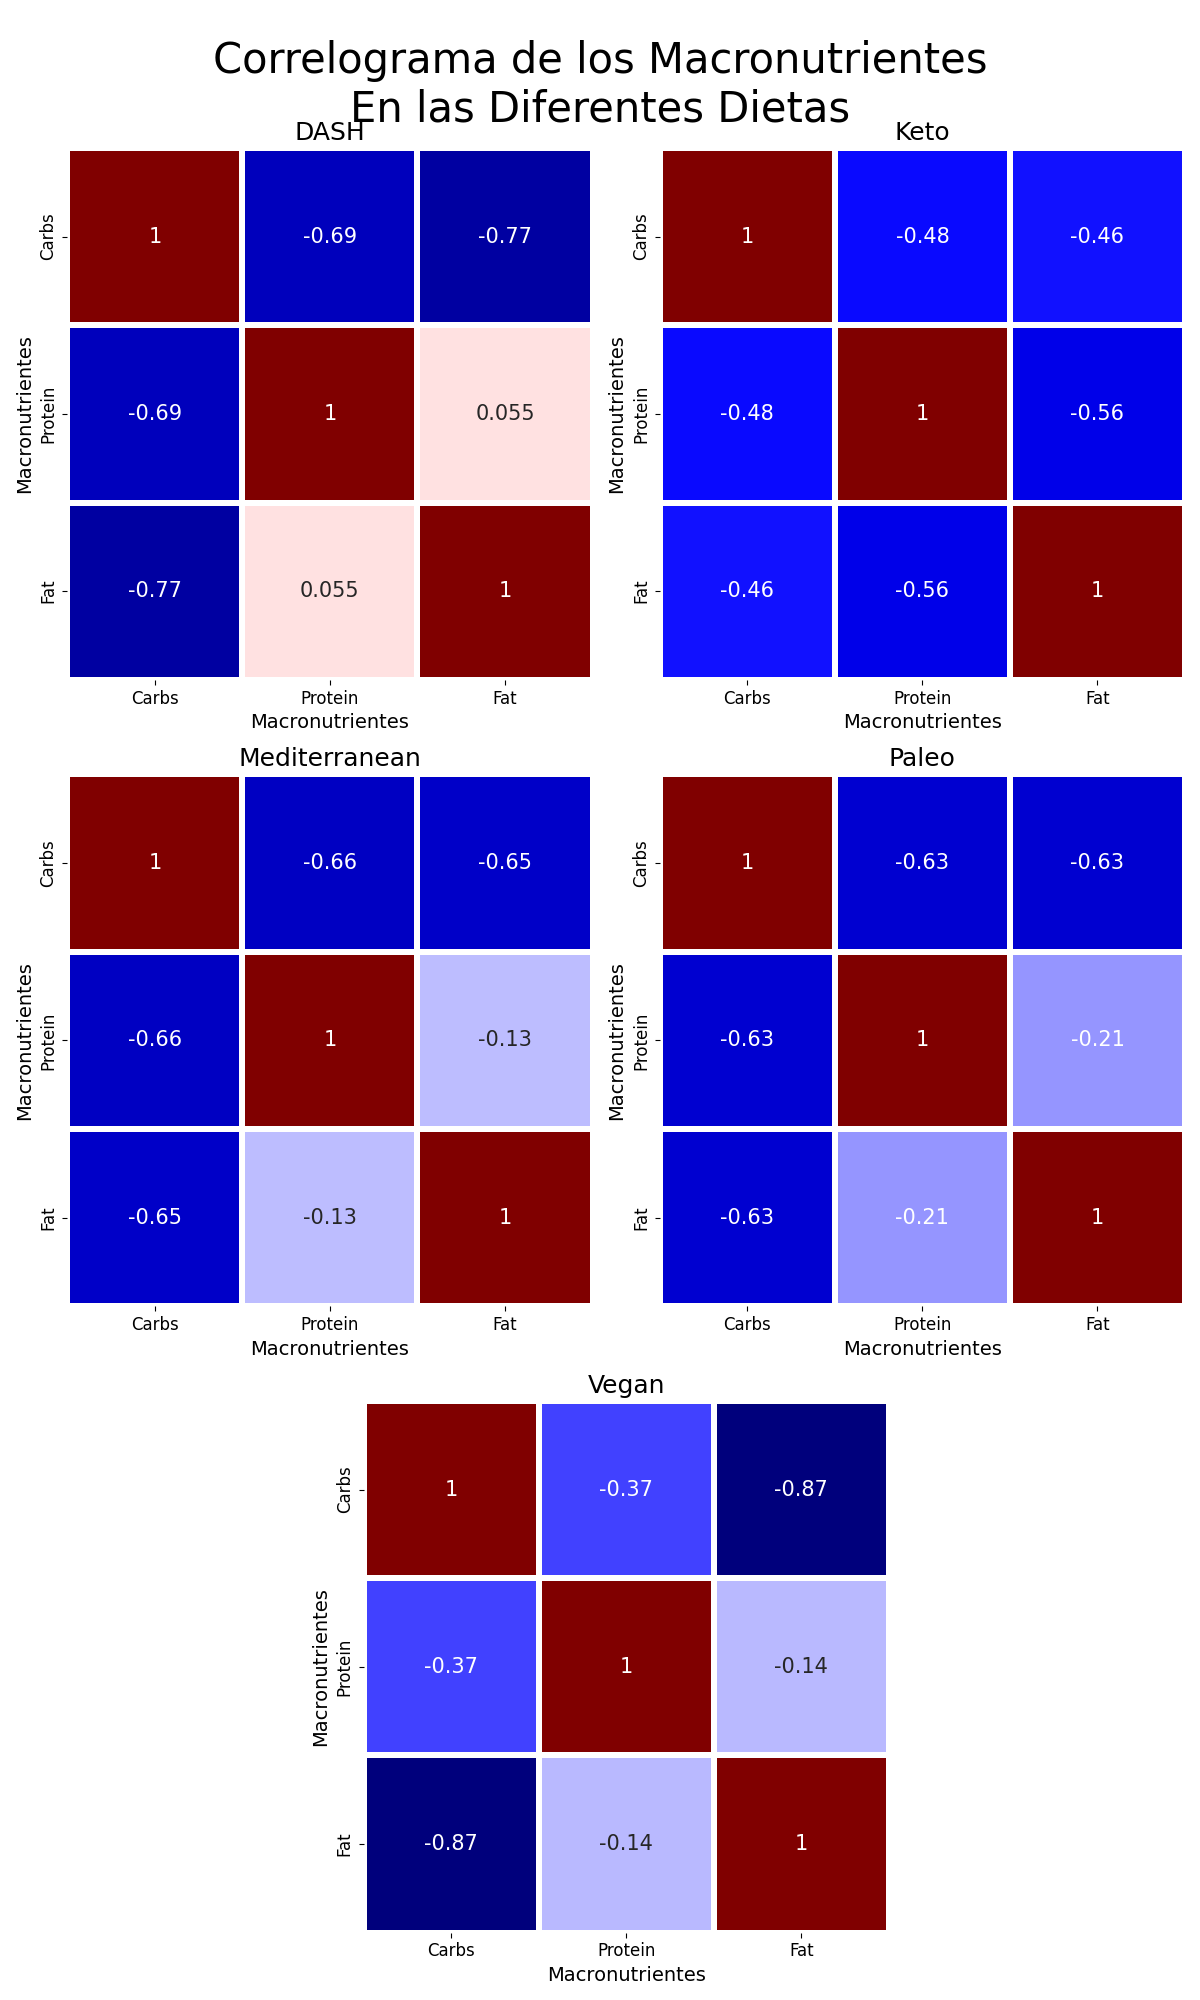
\includegraphics[width=0.8\textwidth]{Resources/Bivariado/Correlation.png}
                \end{center}
            }
        }
    }
        
    \newpage
    
    {
        \printbibliography[heading=bibintoc,title={Referencias Bibliográficas}]
    }

\end{document}